\documentclass[12pt,a4paper]{article}

% Modelo fornecido para o trabalho: manter este arquivo na mesma pasta.
% ===========================================================================
% QUICK EXAMPLES
% ===========================================================================
%
% The examples below show how to use the specification template.
% They can be copied and adapted directly into the main document.
%
% ---------------------------------------------------------------------------
% Functional Requirement
% ---------------------------------------------------------------------------
%
% \fr{User Authentication}{
%     \item The system shall allow users to authenticate using
%     their username and password.
%
%     \item The system shall reject invalid credentials.
%
%     \item The system shall lock the account after three
%     consecutive failed attempts.
% }
%
% ---------------------------------------------------------------------------
% Non-functional Requirement
% ---------------------------------------------------------------------------
%
% \nfr{Authentication Response Time}{
%     \item The system shall authenticate users within 2 seconds
%     under normal operating conditions.
% }
%
% ---------------------------------------------------------------------------
% Use Case
% ---------------------------------------------------------------------------
%
% \begin{usecase}{Perform Login}
%
%     \ucdescription{
%         Allows a user to authenticate into the system using
%         their credentials.
%     }
%
%     \ucactors{
%         \item User
%     }
%
%     \ucpreconditions{
%         \item The user must be registered in the system.
%         \item The system must be available.
%     }
%
%     \ucmainflow{
%         \item The user enters their username and password.
%         \item The system validates the provided credentials.
%         \item The system creates an authenticated session.
%         \item The system grants access to the application.
%     }
%
%     \ucalternativeflow{
%         \item If the credentials are invalid, the system informs
%         the user that the username or password is incorrect.
%
%         \item If the account is locked, the system denies access.
%     }
%
%     \ucbusinessrules{
%         \item The provided password must match the registered password.
%         \item The account is locked after three consecutive failed attempts.
%     }
%
%     \ucpostconditions{
%         \item The user is authenticated.
%         \item An authenticated session exists for the user.
%     }

%     \ucrelatedrequirements{
%         \item FR01
%     }
%
% \end{usecase}
%
% ---------------------------------------------------------------------------
% Operation Contract
% ---------------------------------------------------------------------------
%
% \begin{operationcontract}{Create Order}
%
%     \ocoperation{
%         createOrder(customer)
%     }
%
%     \ocdescription{
%         Creates a new order for the specified customer.
%     }
%
%     \ocpreconditions{
%         \item The customer must exist.
%         \item The customer must be active.
%     }
%
%     \ocpostconditions{
%         \item A new order is created.
%         \item The order is associated with the customer.
%         \item The order status is set to \texttt{OPEN}.
%     }
%
%     \ocrelatedusecases{
%         \item \ref{uc:place-order}
%     }
%
% \end{operationcontract}
%
% ---------------------------------------------------------------------------
% Referencing
% ---------------------------------------------------------------------------
%
% Requirements:
%
% \ref{fr:user-authentication}
% \ref{nfr:authentication-response-time}
%
% Use cases:
%
% \ref{uc:perform-login}
%
% Operation contracts:
%
% \ref{oc:create-order}
%
% The identifiers (FR01, NFR01, UC01, OC01, ...) are generated
% automatically, and labels are generated from the item names.
%
% ===========================================================================


% ===========================================================================
% PACKAGES
% ===========================================================================
\usepackage[utf8]{inputenc}
\usepackage[a4paper,margin=2cm]{geometry}
\usepackage{enumitem}
\usepackage{titlesec}
\usepackage{hyperref}
\usepackage{titling}
\usepackage{graphicx}
\usepackage[most]{tcolorbox}

% ---------------------------------------------------------------------------
% Customizations
% ---------------------------------------------------------------------------

% Subsection formatting
\titleformat{\subsection}
  {\normalfont\large\bfseries}
  {\thesubsection}
  {1em}
  {\underline}

% Itemize formatting
\setlist[itemize,1]{label=$\bullet$}
\setlist[itemize,2]{label=$\circ$}
\setlist[itemize,3]{label=$\diamond$}

% ---------------------------------------------------------------------------
% Title
% ---------------------------------------------------------------------------

\setlength{\droptitle}{-2cm}

\pretitle{\begin{flushleft}\LARGE\bfseries}
\posttitle{\end{flushleft}}

\preauthor{\begin{flushleft}\large}
\postauthor{\end{flushleft}}

\predate{\begin{flushleft}\large}
\postdate{\end{flushleft} \vspace{-1cm}}

% ---------------------------------------------------------------------------
% Requirements
% ---------------------------------------------------------------------------

\newcounter{functionalrequirement}
\newcounter{nonfunctionalrequirement}

% Functional requirement identifier: FR01, FR02, ...
\renewcommand{\thefunctionalrequirement}{%
    FR\ifnum\value{functionalrequirement}<10 0\fi\arabic{functionalrequirement}%
}

% Non-functional requirement identifier: NFR01, NFR02, ...
\renewcommand{\thenonfunctionalrequirement}{%
    NFR\ifnum\value{nonfunctionalrequirement}<10 0\fi\arabic{nonfunctionalrequirement}%
}

\ExplSyntaxOn

% Convert requirement name into a stable label.
\cs_new_protected:Npn \requirement_slug:n #1
{
    % Convert to lowercase.
    \tl_set:Nx \l_tmpa_tl
    {
        \str_lowercase:n { #1 }
    }

    \str_replace_all:Nnn \l_tmpa_tl { á } { a }
    \str_replace_all:Nnn \l_tmpa_tl { à } { a }
    \str_replace_all:Nnn \l_tmpa_tl { â } { a }
    \str_replace_all:Nnn \l_tmpa_tl { ã } { a }
    \str_replace_all:Nnn \l_tmpa_tl { ä } { a }

    \str_replace_all:Nnn \l_tmpa_tl { é } { e }
    \str_replace_all:Nnn \l_tmpa_tl { è } { e }
    \str_replace_all:Nnn \l_tmpa_tl { ê } { e }
    \str_replace_all:Nnn \l_tmpa_tl { ë } { e }

    \str_replace_all:Nnn \l_tmpa_tl { í } { i }
    \str_replace_all:Nnn \l_tmpa_tl { ì } { i }
    \str_replace_all:Nnn \l_tmpa_tl { î } { i }
    \str_replace_all:Nnn \l_tmpa_tl { ï } { i }

    \str_replace_all:Nnn \l_tmpa_tl { ó } { o }
    \str_replace_all:Nnn \l_tmpa_tl { ò } { o }
    \str_replace_all:Nnn \l_tmpa_tl { ô } { o }
    \str_replace_all:Nnn \l_tmpa_tl { õ } { o }
    \str_replace_all:Nnn \l_tmpa_tl { ö } { o }

    \str_replace_all:Nnn \l_tmpa_tl { ú } { u }
    \str_replace_all:Nnn \l_tmpa_tl { ù } { u }
    \str_replace_all:Nnn \l_tmpa_tl { û } { u }
    \str_replace_all:Nnn \l_tmpa_tl { ü } { u }

    \str_replace_all:Nnn \l_tmpa_tl { ç } { c }

    % Replace every sequence of non-alphanumeric characters with '-'.
    \regex_replace_all:nnN
        { [^a-z0-9]+ }
        { - }
        \l_tmpa_tl

    % Remove '-' from the beginning.
    \regex_replace_once:nnN
        { \A-+ }
        { }
        \l_tmpa_tl

    % Remove '-' from the end.
    \regex_replace_once:nnN
        { -+\Z }
        { }
        \l_tmpa_tl
}

% Functional requirement
\NewDocumentCommand{\fr}{m +m}
{
    \refstepcounter{functionalrequirement}
    \noindent
    \textbf{\thefunctionalrequirement{} - #1}
    \requirement_slug:n { #1 }
    \exp_args:Nx \label { fr:\l_tmpa_tl }

    \begin{itemize}[noitemsep, topsep=2pt, leftmargin=2em]
        #2
    \end{itemize}

    \par\medskip
}

% Non-functional requirement
\NewDocumentCommand{\nfr}{m +m}
{
    \refstepcounter{nonfunctionalrequirement}
    \noindent
    \textbf{\thenonfunctionalrequirement{} - #1}
    \requirement_slug:n { #1 }
    \exp_args:Nx \label { nfr:\l_tmpa_tl }

    \begin{itemize}[noitemsep, topsep=2pt, leftmargin=2em]
        #2
    \end{itemize}

    \par\medskip
}

\ExplSyntaxOff

% ---------------------------------------------------------------------------
% Use Cases
% ---------------------------------------------------------------------------

\newcounter{usecase}

% Use case identifier: UC01, UC02, ...
\renewcommand{\theusecase}{%
    UC\ifnum\value{usecase}<10 0\fi\arabic{usecase}%
}

% Use case box
\newtcolorbox{usecasebox}{
    enhanced,
    breakable,
    lines before break=15,
    colback=white,
    colframe=black!40,
    boxrule=0.5pt,
    arc=2pt,
    left=8pt,
    right=8pt,
    top=6pt,
    bottom=6pt,
    before skip=8pt,
    after skip=12pt,
    segmentation style={
        line width=0.5pt,
        solid
    }
}

\ExplSyntaxOn

% Use case environment
\NewDocumentEnvironment{usecase}{m}
{
    \refstepcounter{usecase}

    % Generate stable label from the use case name.
    \requirement_slug:n { #1 }
    \exp_args:Nx \label { uc:\l_tmpa_tl }

    % Compact title, similar to requirements.
    \begin{usecasebox}
    \noindent
    \textbf{\theusecase{} - #1}
    \par\smallskip
    \tcblower
}
{
    \end{usecasebox}
}

\ExplSyntaxOff

% Use Case Fields ----------------------------------------
\newcommand{\ucdescription}[1]{
    \noindent
    \textbf{Description}
    \par
    \leftskip=1em
    #1
    \par
    \leftskip=0pt
    \medskip
}

\newcommand{\ucactors}[1]{
    \noindent
    \textbf{Actors}
    \begin{itemize}[noitemsep, topsep=2pt, leftmargin=2em]
        #1
    \end{itemize}
}

\newcommand{\ucrelatedrequirements}[1]{
    \noindent
    \textbf{Related requirements}
    \begin{itemize}[noitemsep, topsep=2pt, leftmargin=2em]
        #1
    \end{itemize}
}

\newcommand{\ucpreconditions}[1]{
    \noindent
    \textbf{Preconditions}
    \begin{itemize}[noitemsep, topsep=2pt, leftmargin=2em]
        #1
    \end{itemize}
}

\newcommand{\ucmainflow}[1]{
    \noindent
    \textbf{Main Flow}
    \begin{enumerate}[noitemsep, topsep=2pt, leftmargin=2.4em]
        #1
    \end{enumerate}
}

\newcommand{\ucalternativeflow}[1]{
    \noindent
    \textbf{Alternative Flows}
    \begin{itemize}[noitemsep, topsep=2pt, leftmargin=2em]
        #1
    \end{itemize}
}

\newcommand{\ucbusinessrules}[1]{
    \noindent
    \textbf{Business Rules}
    \begin{itemize}[noitemsep, topsep=2pt, leftmargin=2em]
        #1
    \end{itemize}
}

\newcommand{\ucpostconditions}[1]{
    \noindent
    \textbf{Postconditions}
    \begin{itemize}[noitemsep, topsep=2pt, leftmargin=2em]
        #1
    \end{itemize}
}

% ---------------------------------------------------------------------------
% Operation Contracts
% ---------------------------------------------------------------------------

\newcounter{operationcontract}

% Operation contract identifier: OC01, OC02, ...
\renewcommand{\theoperationcontract}{%
    OC\ifnum\value{operationcontract}<10 0\fi\arabic{operationcontract}%
}

% Operation contract box
\newtcolorbox{operationcontractbox}{
    enhanced,
    breakable,
    lines before break=15,
    colback=white,
    colframe=black!40,
    boxrule=0.5pt,
    arc=2pt,
    left=8pt,
    right=8pt,
    top=6pt,
    bottom=6pt,
    before skip=8pt,
    after skip=12pt,
    segmentation style={
        line width=0.3pt,
        draw=black!30
    }
}

\ExplSyntaxOn

% Operation contract environment
\NewDocumentEnvironment{operationcontract}{m}
{
    \refstepcounter{operationcontract}

    % Generate stable label from the operation contract name.
    \requirement_slug:n { #1 }
    \exp_args:Nx \label { oc:\l_tmpa_tl }

    \begin{operationcontractbox}
        \noindent
        \textbf{\theoperationcontract{} - #1}

        \tcblower
}
{
    \end{operationcontractbox}
}

\ExplSyntaxOff

% Operation Contract Fields ------------------------------------------
\newcommand{\ocoperation}[1]{
    \noindent
    \textbf{Operation}
    \par
    \leftskip=1em
    \texttt{#1}
    \par
    \leftskip=0pt
    \medskip
}

\newcommand{\ocdescription}[1]{
    \noindent
    \textbf{Description}
    \par
    \leftskip=1em
    #1
    \par
    \leftskip=0pt
    \medskip
}

\newcommand{\ocpreconditions}[1]{
    \noindent
    \textbf{Preconditions}
    \begin{itemize}[noitemsep, topsep=2pt, leftmargin=2em]
        #1
    \end{itemize}
}

\newcommand{\ocpostconditions}[1]{
    \noindent
    \textbf{Postconditions}
    \begin{itemize}[noitemsep, topsep=2pt, leftmargin=2em]
        #1
    \end{itemize}
}

\newcommand{\ocrelatedusecases}[1]{
    \noindent
    \textbf{Related Use Cases}
    \begin{itemize}[noitemsep, topsep=2pt, leftmargin=2em]
        #1
    \end{itemize}
}

\usepackage[T1]{fontenc}
\usepackage{float}
\usepackage[brazilian]{babel}
\setlength{\parindent}{0pt}
\setlength{\parskip}{3pt plus 1pt minus 1pt}
\hypersetup{hidelinks,pdftitle={TP2: Refatoracao de um Sistema de Geracao de Relatorios},pdflang={pt-BR}}
\setlength{\emergencystretch}{4em}

\title{TP2: Refatoração de um Sistema de Geração de Relatórios}
\author{\small
	Bruno Aquiles de Lima\\
	Bruno S. Vila Lobos\\
	Luiz Henrique Murback Wiedmer
}
\date{}

\begin{document}
	\maketitle
	\tableofcontents
	\vspace{5pt}
	\small
	
	\section{Introdução}
	Este trabalho apresenta o projeto de refatoração de um sistema gerador de relatórios de cidades. Na versão original, o programa estava rigidamente acoplado a um arquivo JSON de caminho fixo e gerava apenas saídas em HTML e TXT. O objetivo desta refatoração é modernizar a arquitetura do sistema preservando as funcionalidades originais e suportando novas fontes e formatos de maneira flexível.
	
	Para atingir esse objetivo, as classes originais, que tinham um grande número de responsabilidades, foram substituídas por componentes modulares, dividindo o sistema em quatro pilares principais: \textbf{leitura, interpretação, formatação e coordenação}.
	
	\section{Implementação original}
	
	O código original sofria com alta duplicação e baixo isolamento de responsabilidades. As classes \texttt{CidadesHTMLReport} e \texttt{CidadesTXTReporter} possuíam estruturas e fluxos de execução praticamente idênticos, como ilustrado nas Figuras \ref{fig:dia_cla_orig}, \ref{fig:dia_seq_html} e \ref{fig:dia_seq_txt}. 

	Além disso, cada classe acumulava tarefas muito distintas: acessar o arquivo, interpretar o conteúdo e apresentar os dados. Esse alto acoplamento tornava a adição de novos formatos um processo complexo, exigindo alterações em várias partes do sistema, inclusive no arquivo \texttt{index.js}, que operava com caminhos fixos e condicionais repetitivas.
	\begin{figure}[!ht]
		\centering
		\caption{Diagrama de classes original}
		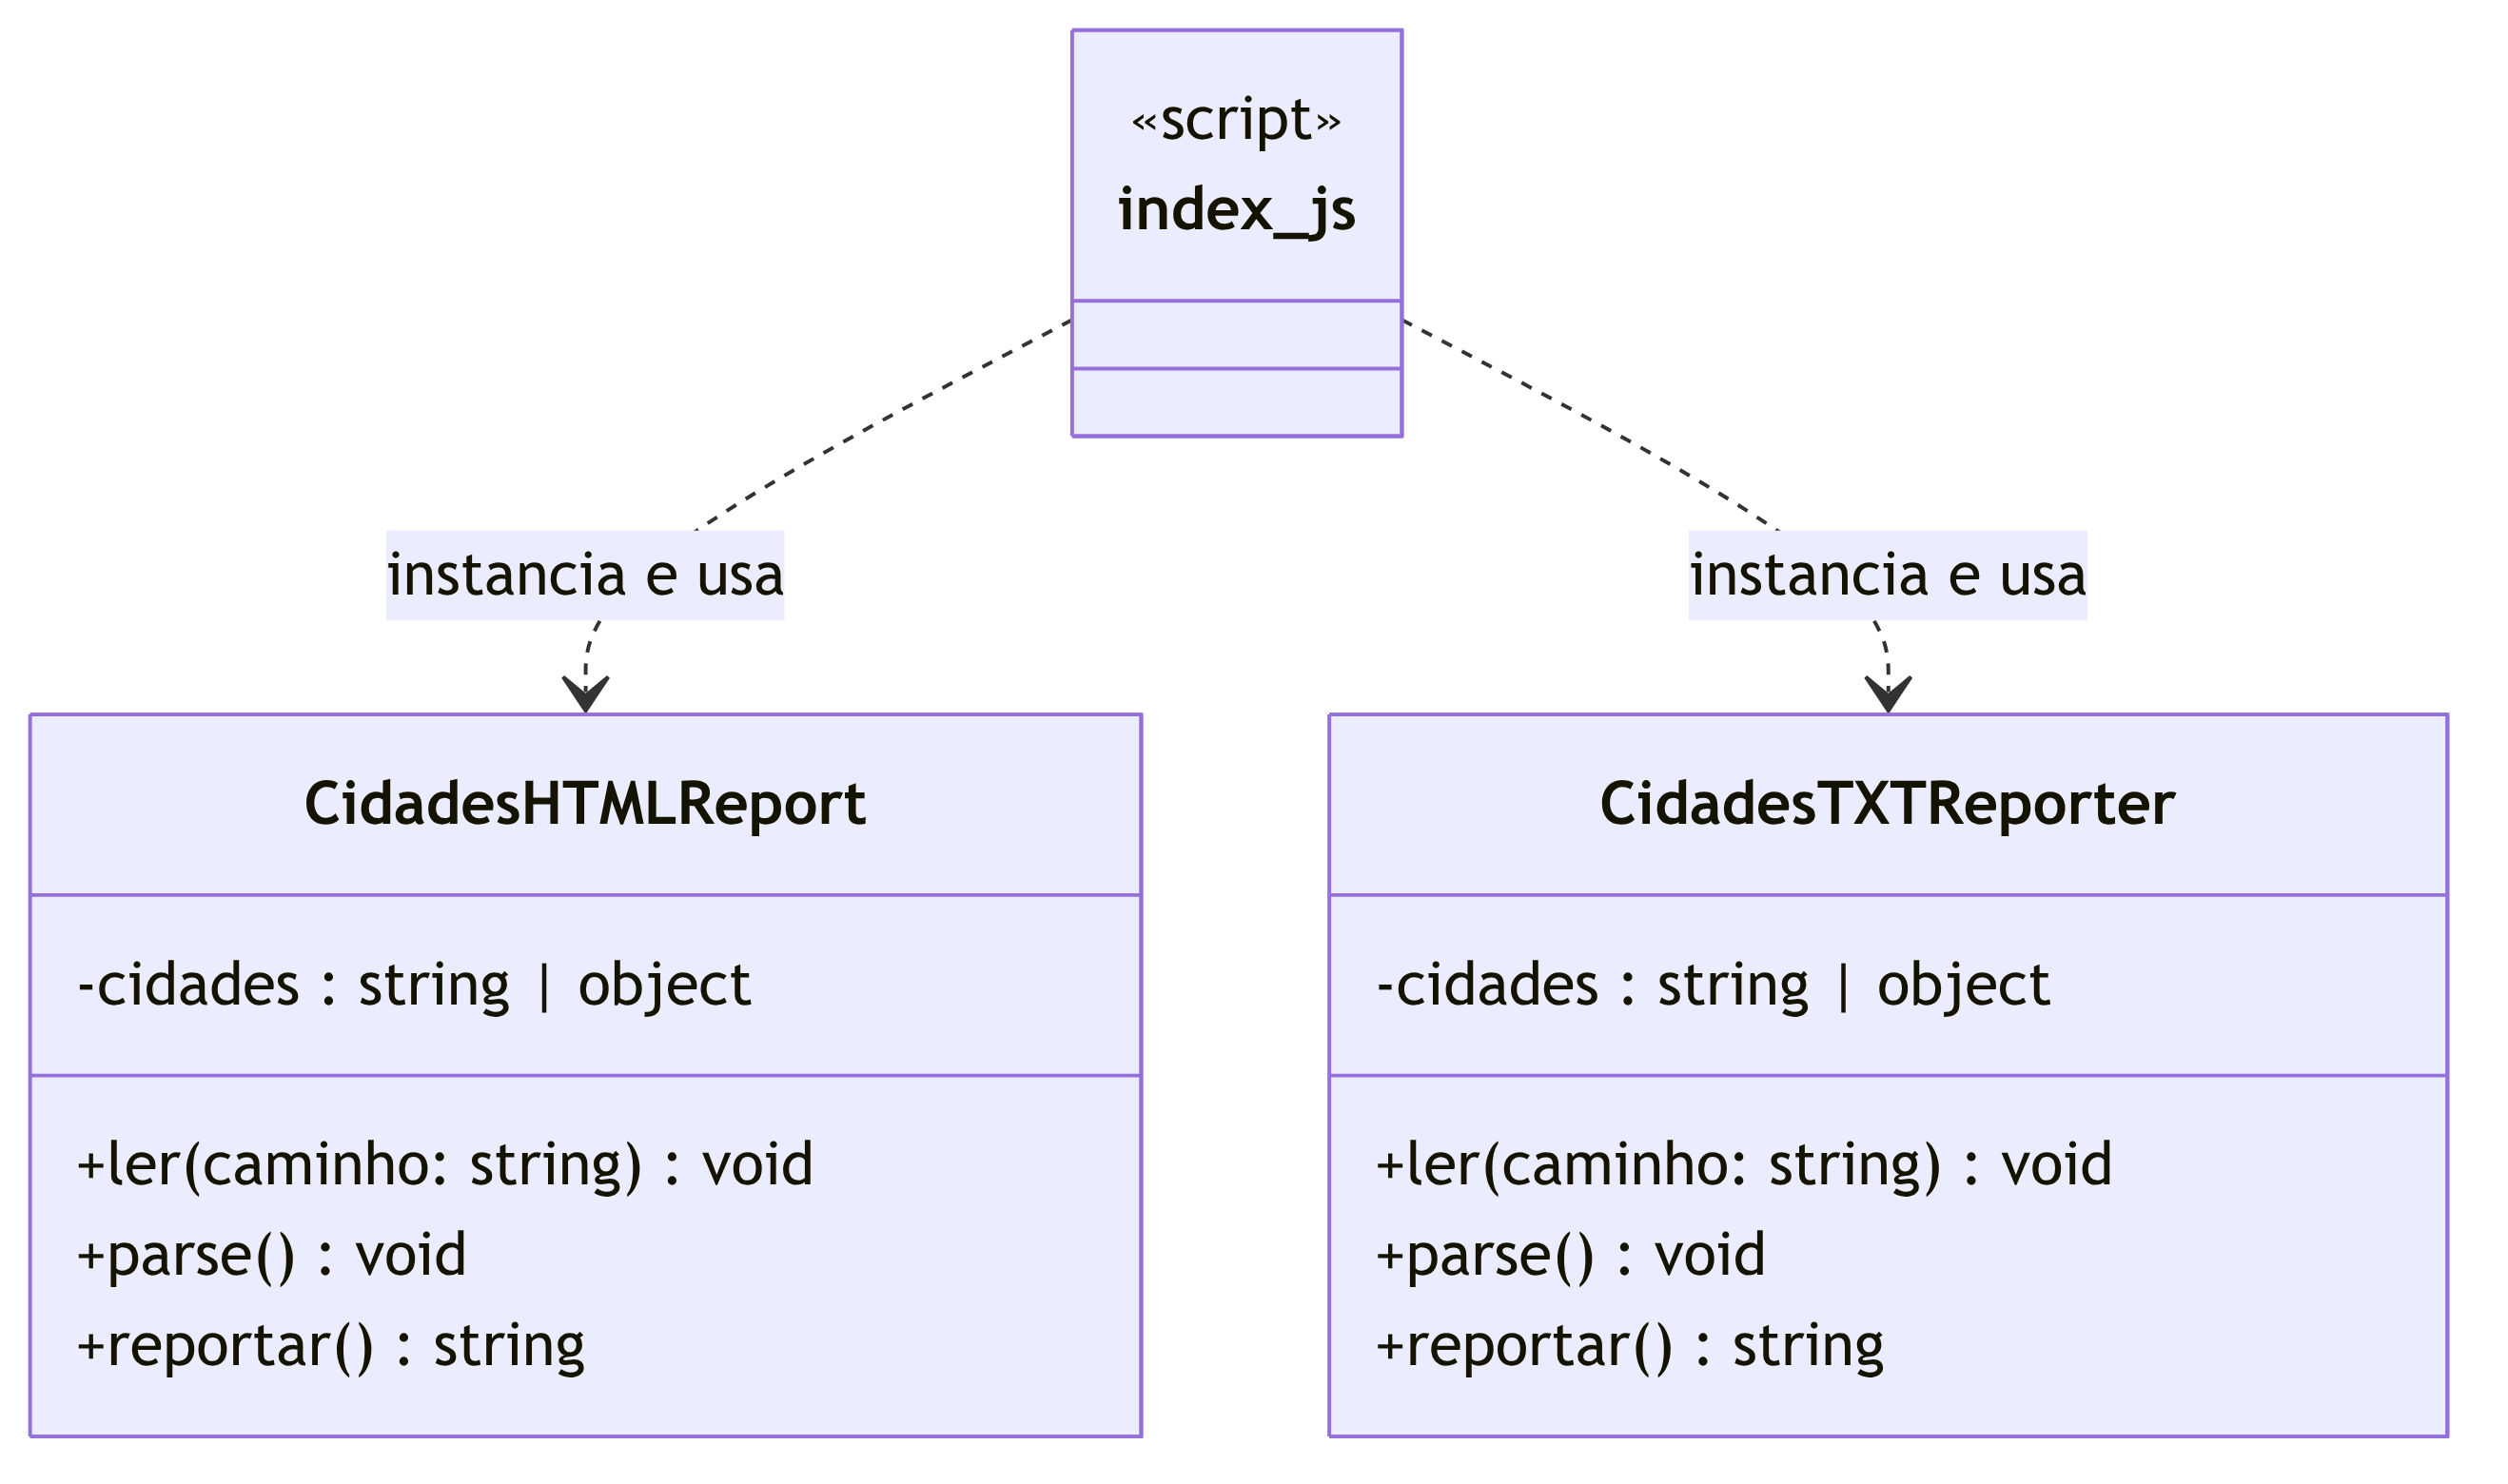
\includegraphics[width=0.8\textwidth]{diagramas/diagrama_classes_orig.png}
		\label{fig:dia_cla_orig}
	\end{figure}
	
	\begin{figure}[!ht]
		\centering
		\caption{Diagrama de sequência original para geração de html}
		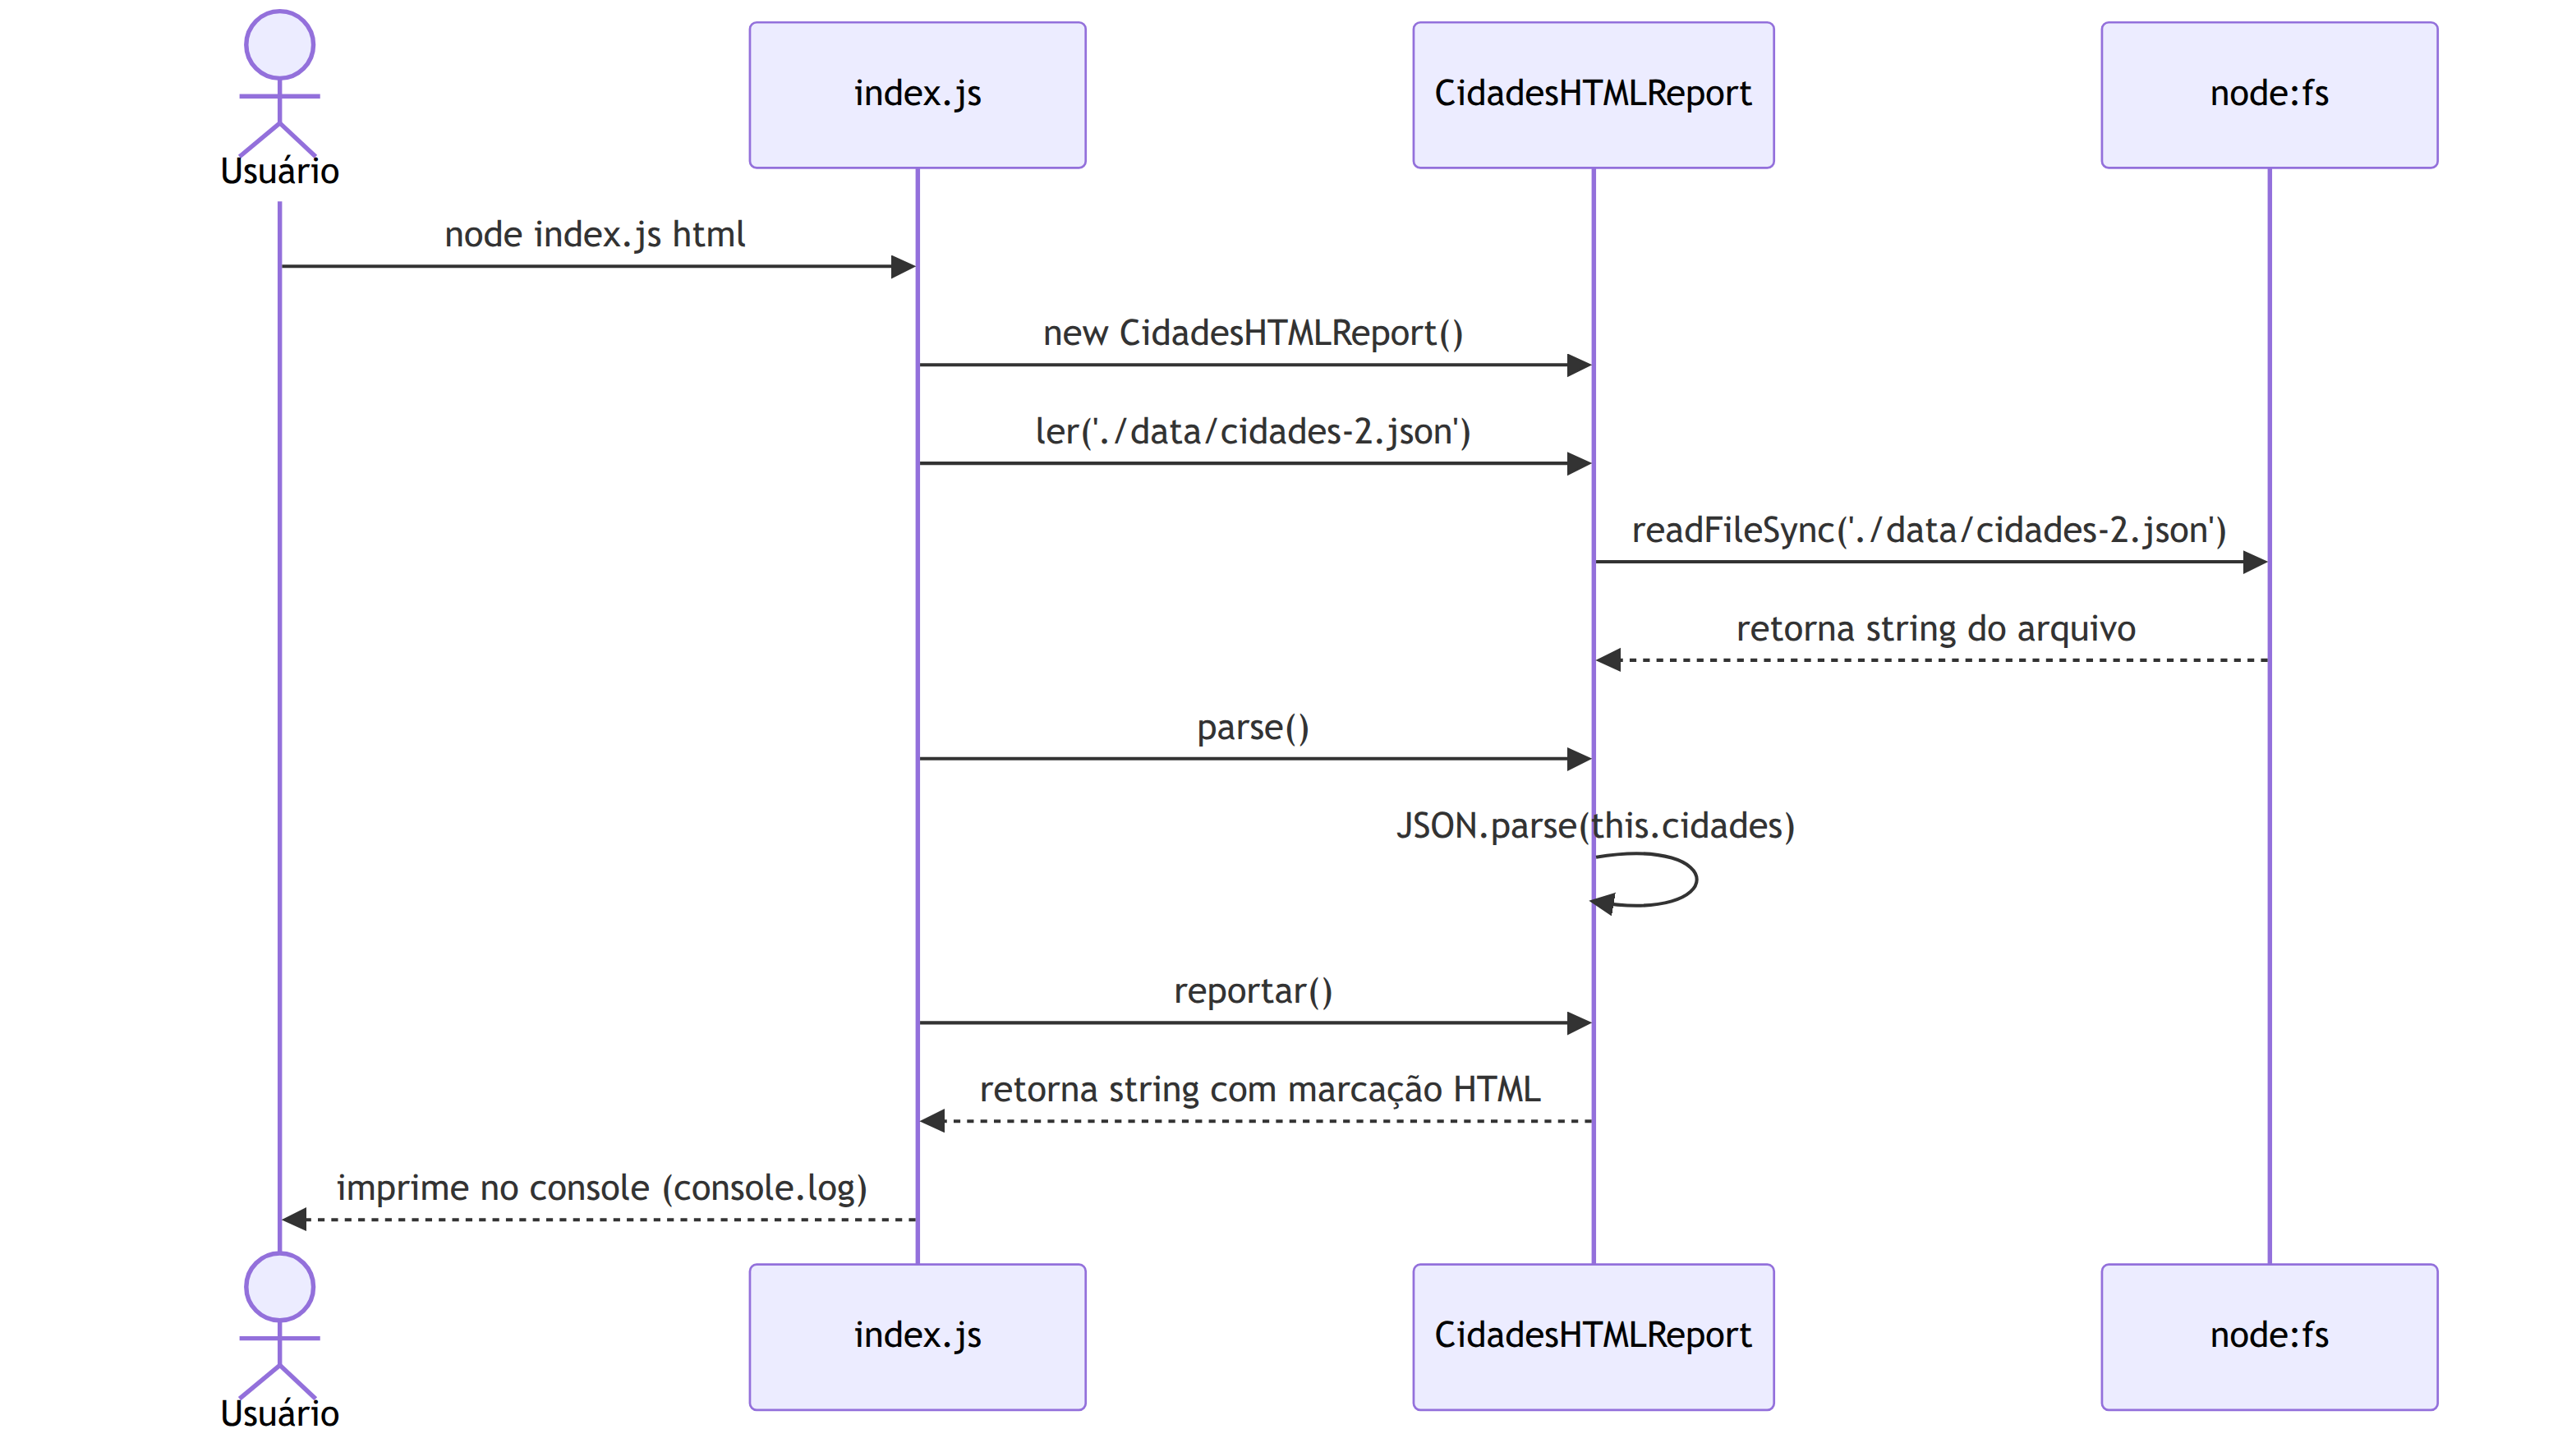
\includegraphics[width=\textwidth]{diagramas/diagrama_seq_orig_html.png}
		\label{fig:dia_seq_html}
	\end{figure}
	
\clearpage
	\begin{figure}[!ht]
		\centering
		\caption{Diagrama de sequência original para geração de txt}
		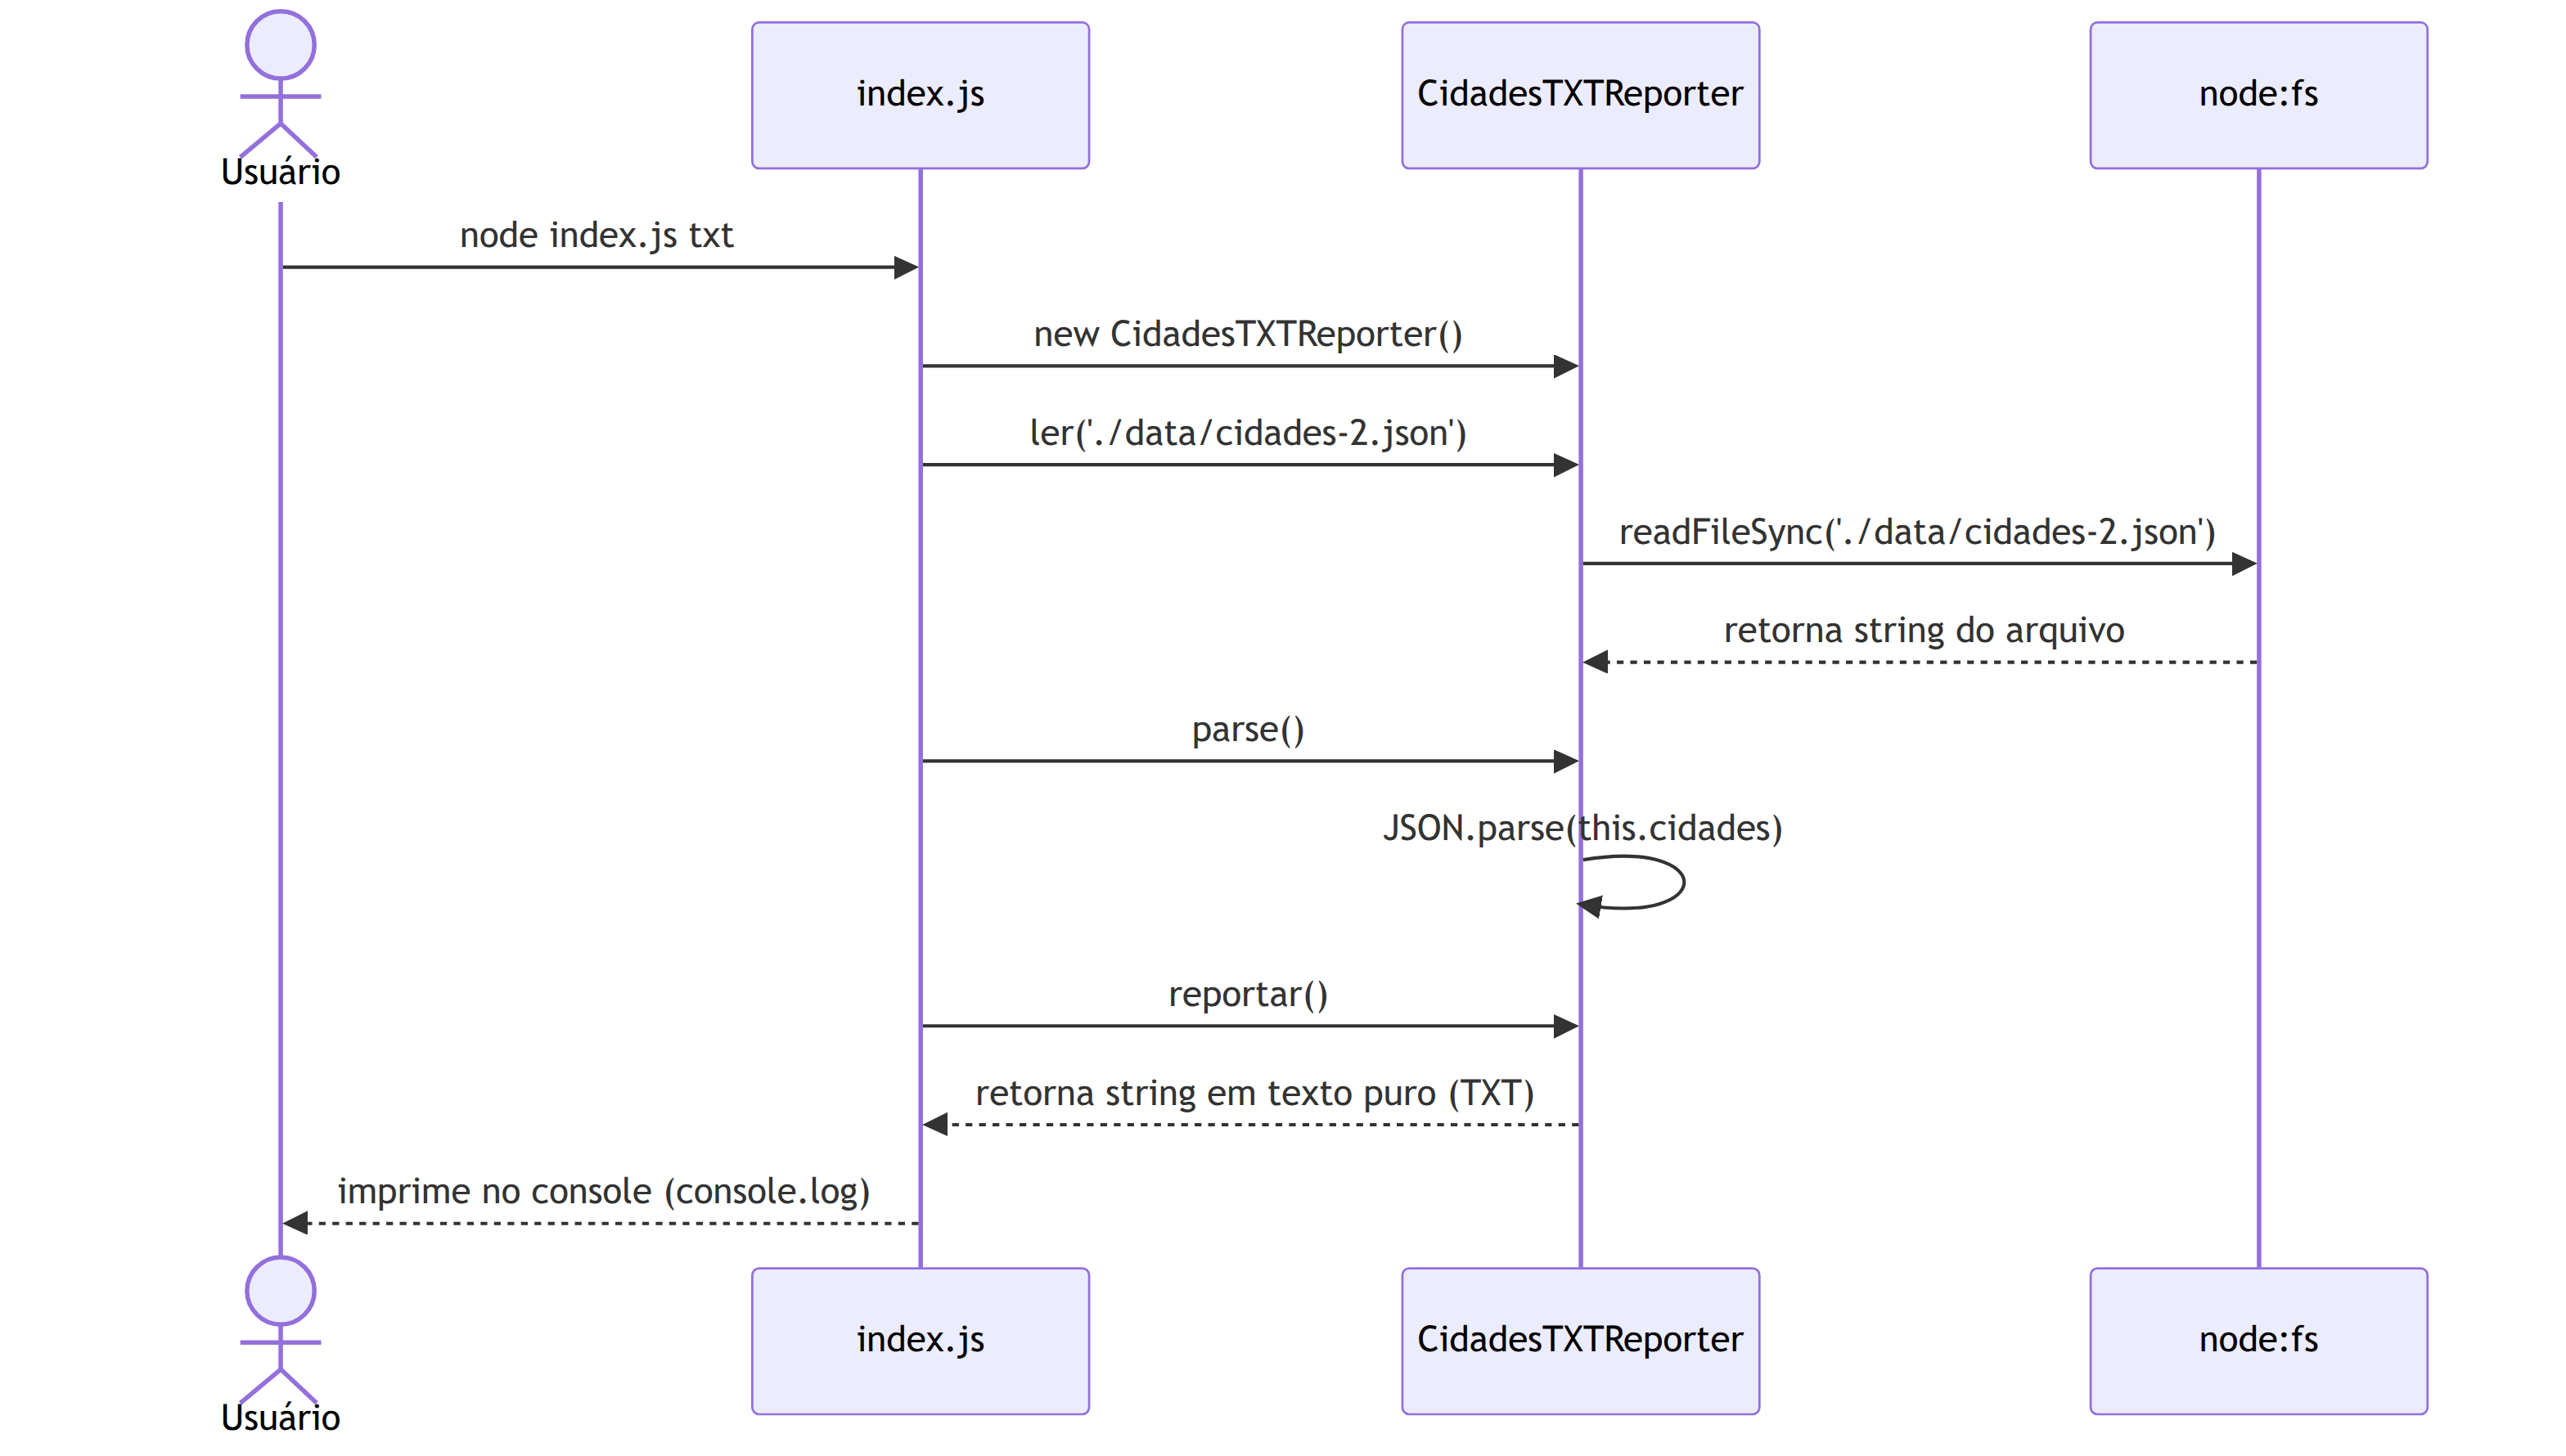
\includegraphics[width=\textwidth]{diagramas/diagrama_seq_orig_txt.png}
		\label{fig:dia_seq_txt}
	\end{figure}

    \section{Refatorações realizadas}
	
	Para resolver os problemas identificados, foi aplicado um conjunto de refatorações focadas em modularidade e flexibilidade, resumidas a seguir.
	
	\subsection{Abstração e Especialização da Leitura}
	A etapa de acesso aos arquivos foi extraída para a classe base \texttt{ILeitor}. Seu método \texttt{ler(caminho)} centraliza a leitura em disco e repassa o conteúdo para o método \texttt{parse(conteudo)}, eliminando a duplicação dessa lógica. 
	
	Como \texttt{ILeitor} atua como uma abstração, suas subclasses (\texttt{LeitorJSON} e \texttt{LeitorCSV}) focam apenas em interpretar o texto recebido e entregá-lo em um formato interno padronizado. Assim, a origem dos dados deixou de ditar o formato do relatório.
	
	\subsection{Formatação Independente}
	A apresentação dos dados foi isolada em formatadores independentes: \texttt{FormatadorHTML}, \texttt{FormatadorTXT} e \texttt{FormatadorCSV}. Todos estendem a abstração \texttt{IFormatador} e implementam o método \texttt{formatar(dados)}. Dessa forma, as classes de saída apenas recebem os dados já procesados e geram o relatório, sem saber ou se importar de onde eles vieram.
	
	\subsection{Coordenação e Ponto de Entrada dinâmico}
	Foi introduzida a classe \texttt{GeradorDeRelatorio}, cuja única função é orquestrar o processo. Ela recebe um leitor e um formatador em seu construtor e, no método \texttt{gerar(caminho)}, faz a ponte entre a obtenção dos dados e a sua formatação. Essa composição reduz o acoplamento drasticamente.
	
	Paralelamente, o \texttt{index.js} foi reescrito. Agora, ele captura os argumentos da linha de comando (\texttt{process.argv}), instancia dinamicamente o leitor e o formatador correspondentes às escolhas do usuário e os injeta no gerador, sem processar nenhum dado diretamente.
	
	\subsection{Tratamento de Erros e Correções}
	Aproveitou-se a refatoração para corrigir um \textit{bug} visual no \texttt{FormatadorTXT}, onde a primeira cidade aparecia colada ao cabeçalho. O \texttt{index.js} também foi blindado: entradas inválidas agora informam o modo correto de uso e encerram a execução graciosamente. Toda a geração foi encapsulada em blocos \texttt{try/catch}, disparando mensagens de erro limpas via \texttt{console.error()} para não corromper a saída de relatórios redirecionados no terminal.
	
	\section{Arquitetura e Padrões de Projeto}
	
	A nova arquitetura (Figuras \ref{fig:dia_cla_mod} e \ref{fig:dia_seq_mod}) substitui o modelo anterior por uma composição de componentes dinâmicos, fortemente ancorada em dois padrões de projeto:
	
	\subsection{Template Method}
	O padrão Template Method foi aplicado na classe \texttt{ILeitor}. O método \texttt{ler()} define o "esqueleto" do algoritmo (abrir e ler o arquivo), enquanto a etapa variável, a conversão dos dados, é delegada às subclasses através do método \texttt{parse()}.
	
	\subsection{Strategy}
	O padrão Strategy foi a base para a classe \texttt{GeradorDeRelatorio}. O gerador enxerga apenas abstrações, de forma que os leitores e formatadores injetados são estratégias intercambiáveis. O sistema agora pode, por exemplo, gerar um relatório CSV a partir de um JSON sem exigir nenhuma mudança em seu núcleo operacional.
	
	\begin{figure}[H]
		\centering
		\caption{Diagrama de classes após refatoração}
		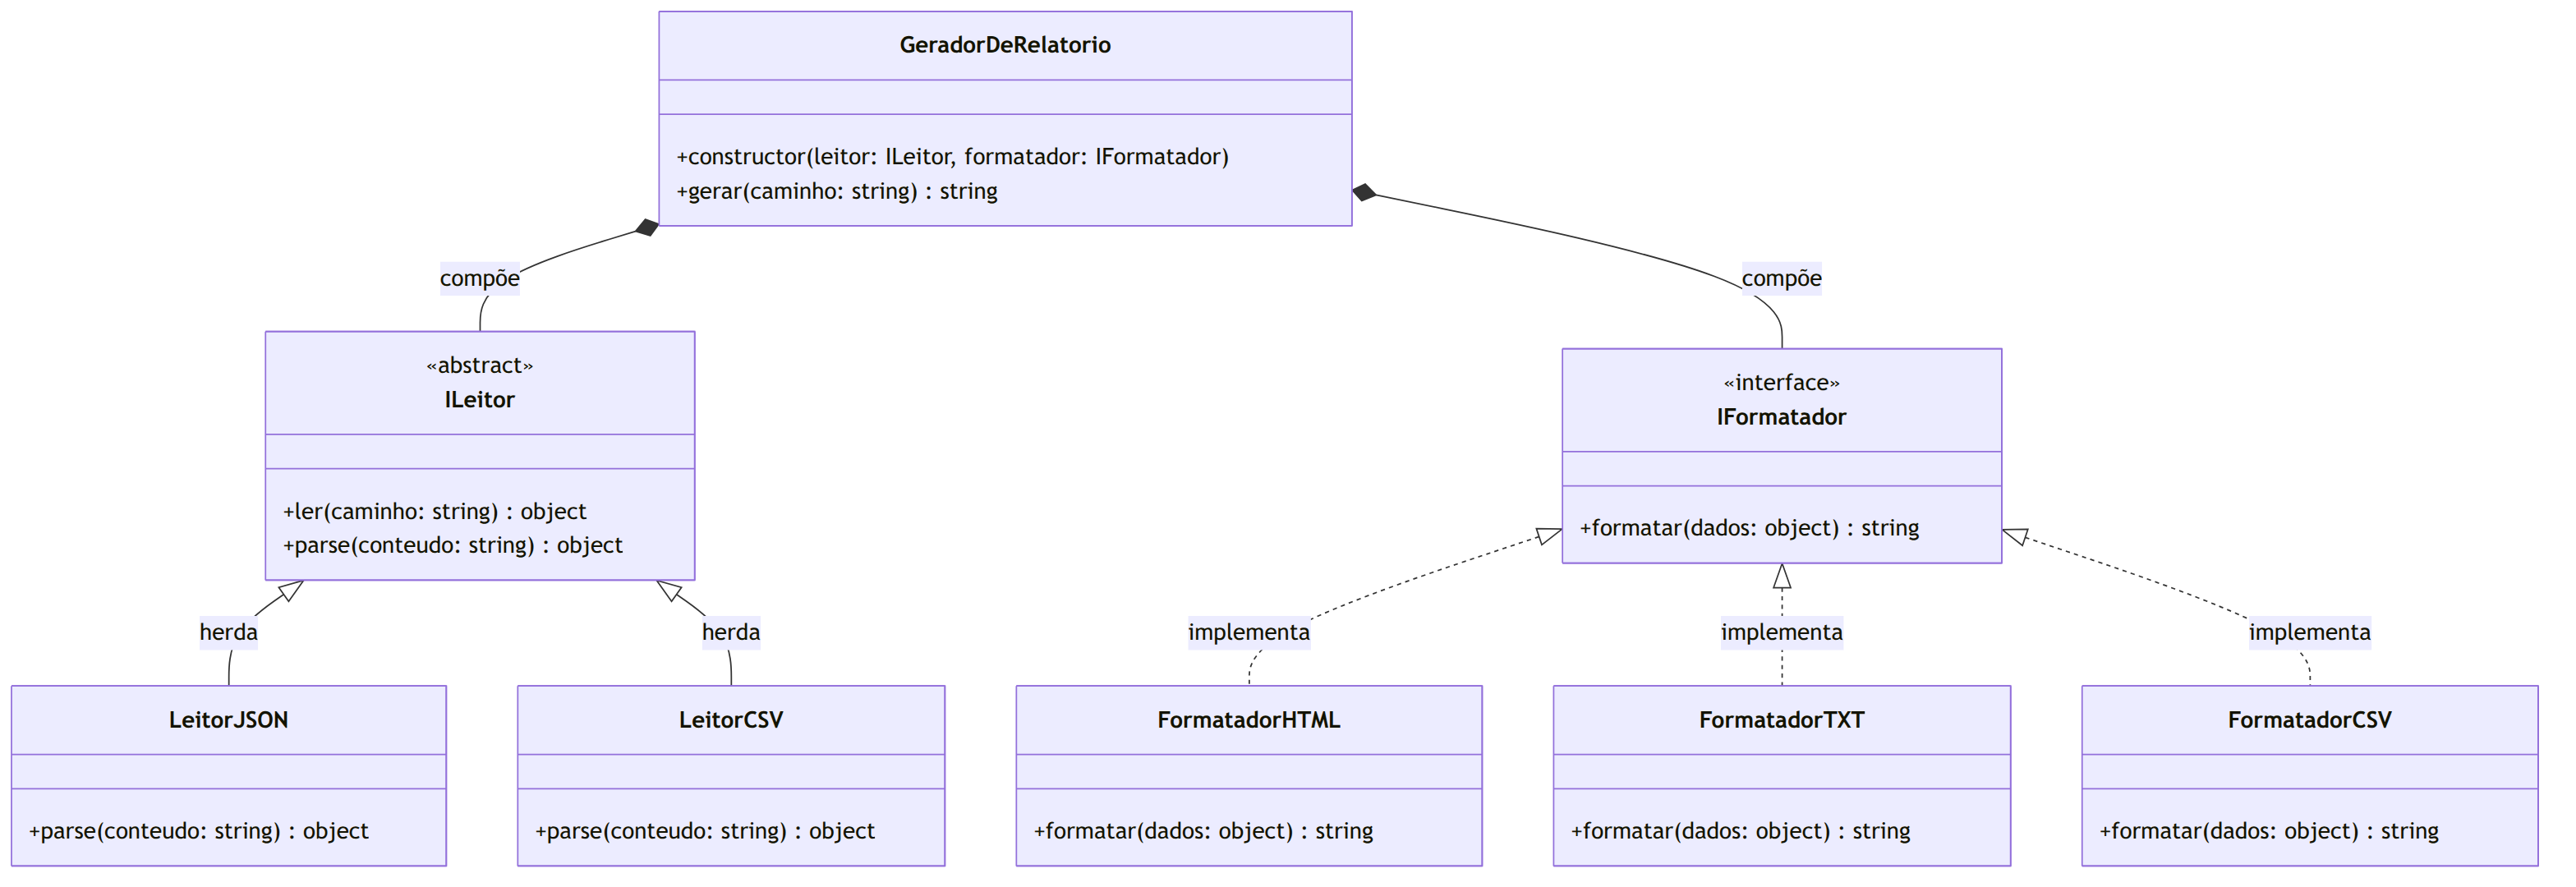
\includegraphics[width=\textwidth]{diagramas/diagrama_classes_mod.png}
		\label{fig:dia_cla_mod}
	\end{figure}
	
	\begin{figure}[H]
		\centering
		\caption{Diagrama de sequência após refatoração}
		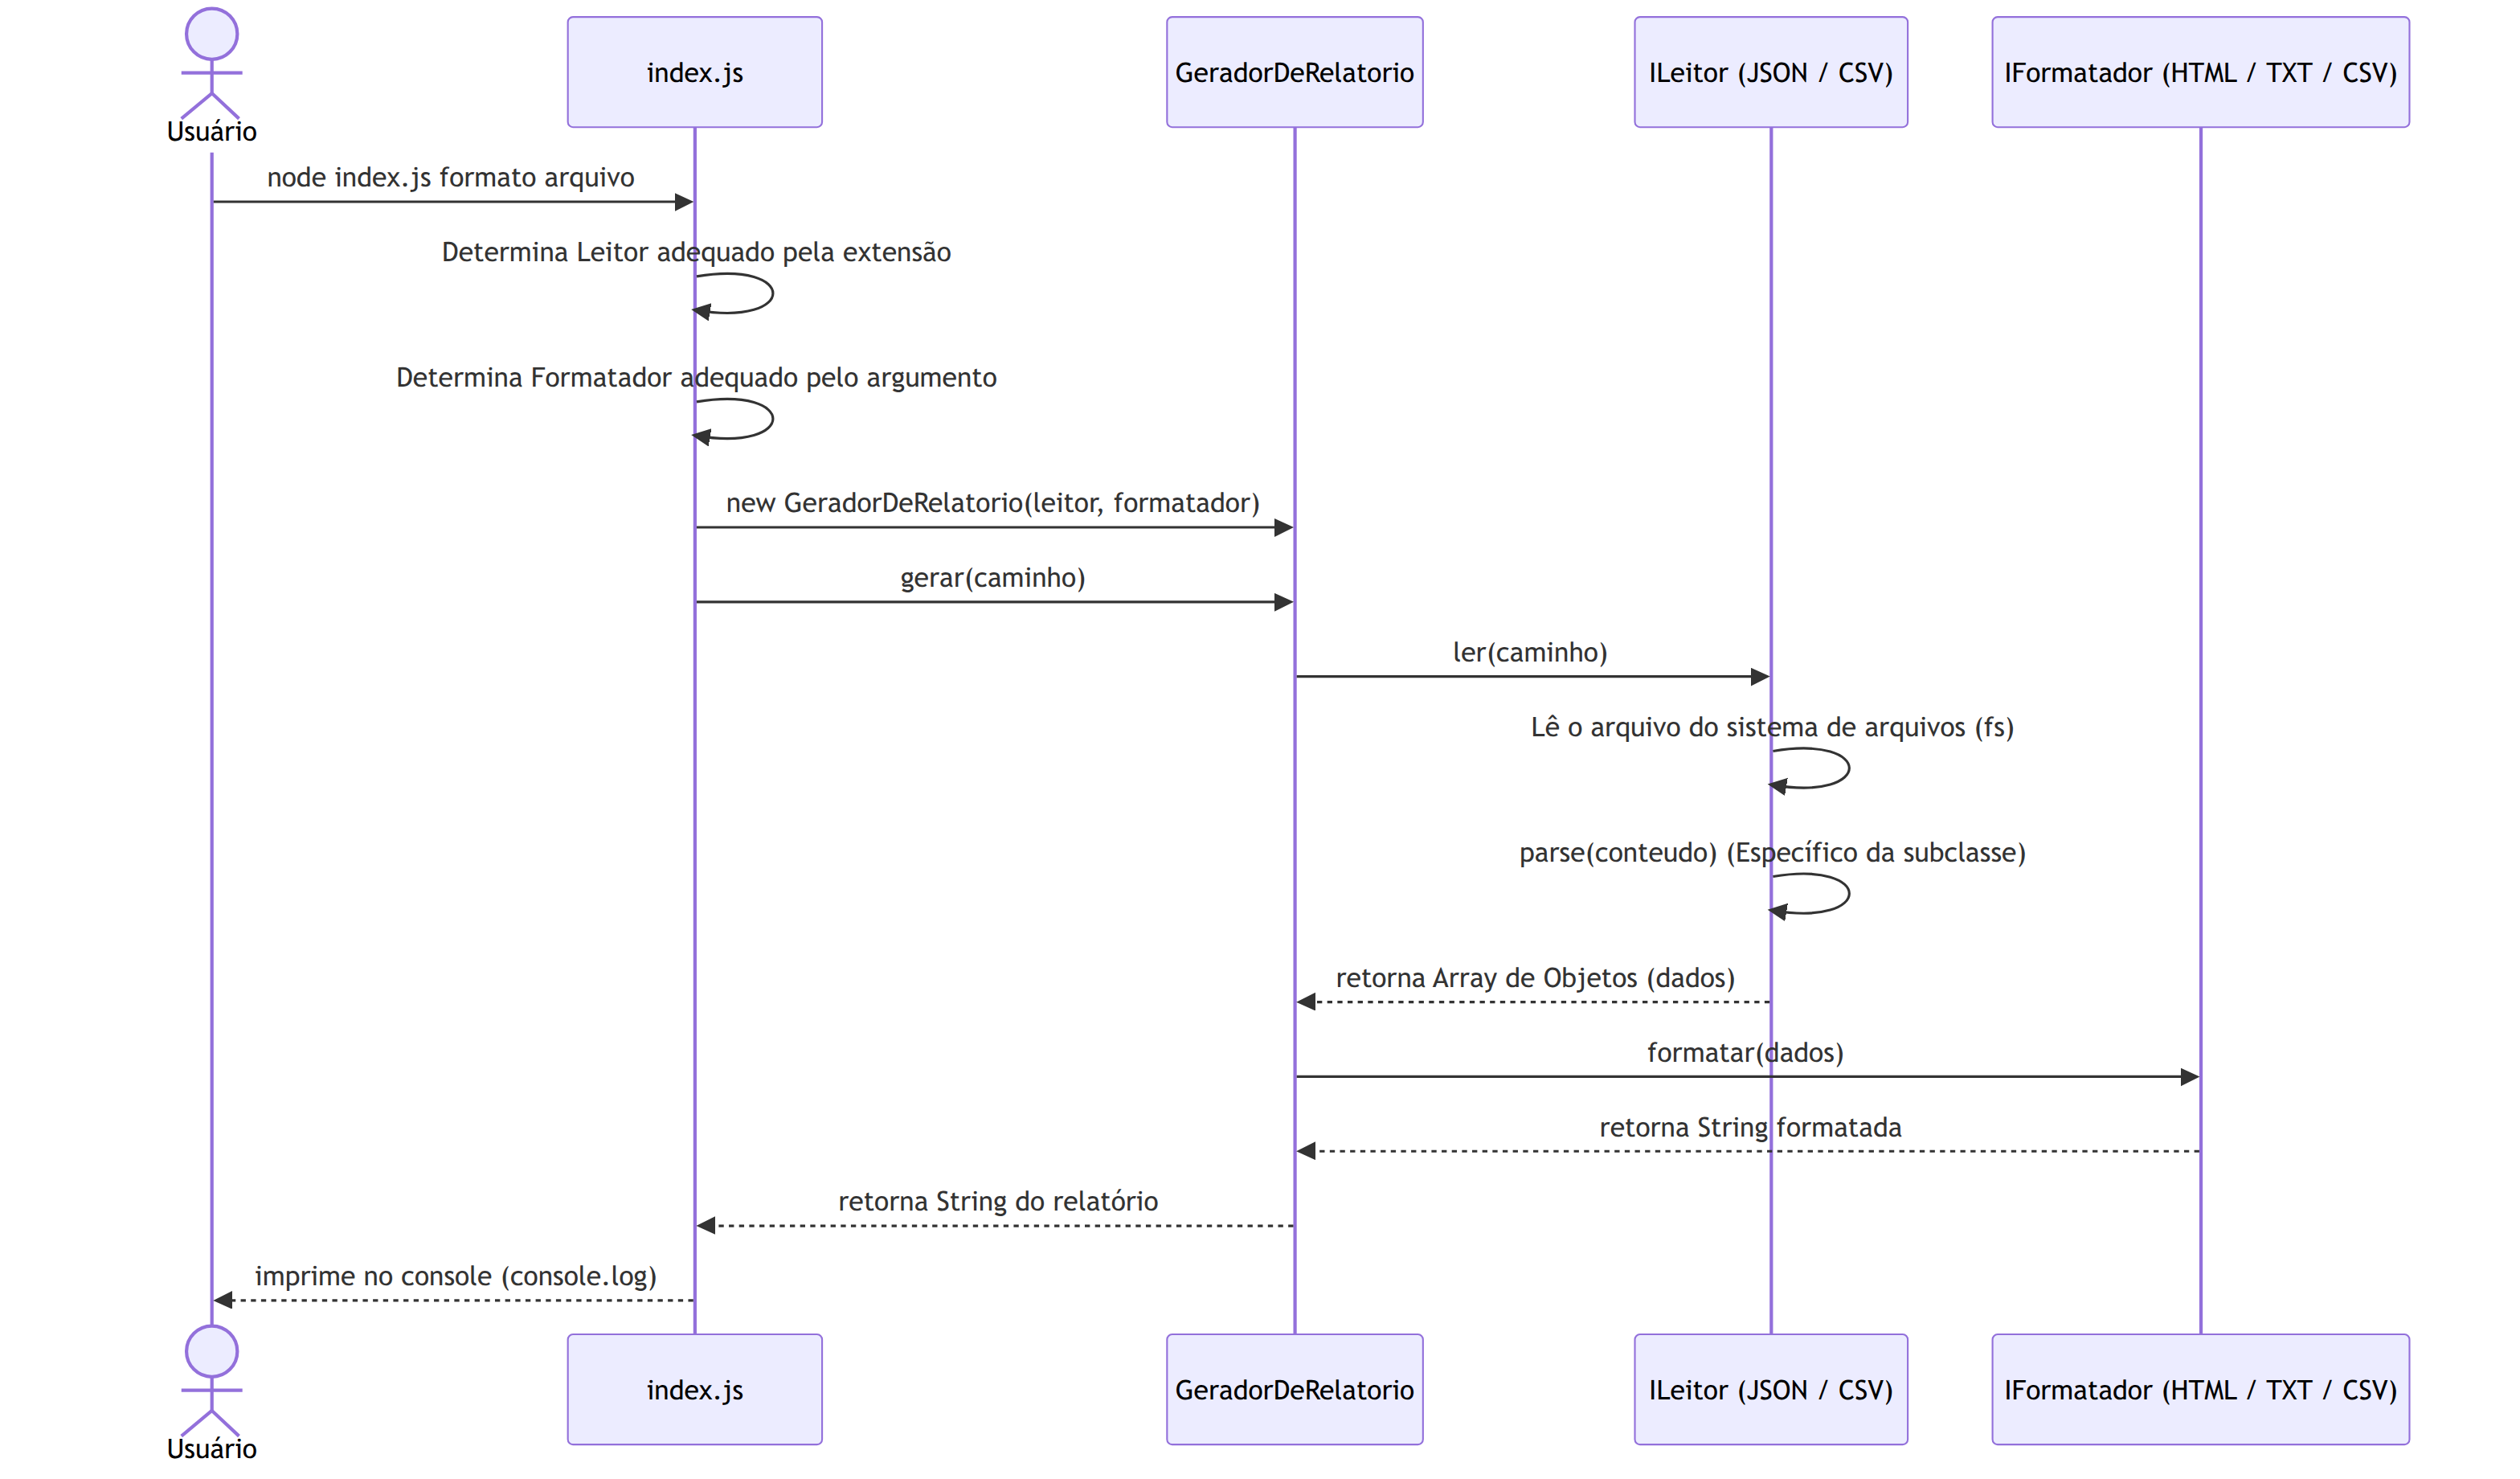
\includegraphics[width=\textwidth]{diagramas/diagrama_seq_mod.png}
		\label{fig:dia_seq_mod}
	\end{figure}
	
	Em resumo, o padrão Strategy foi usado como estrutura geral e o Template Method para simplificar a implementação da leitura dos dados.
	
	\section{Relação com os princípios SOLID}
	
	A reestruturação do código foi guiada pelas boas práticas do SOLID, como apresentado a seguir:
	
	\begin{itemize}
		\item \textbf{SRP (Responsabilidade Única):} Cada componente tem apenas um objetivo. Leitores apenas leem; formatadores apenas formatam; o gerador apenas orquestra.
		\item \textbf{OCP (Aberto/Fechado):} É fácil adicionar novos formatos. Um \texttt{FormatadorMarkdown}, por exemplo, pode ser adicionado ao sistema sem alterar os arquivos do gerador ou dos leitores existentes.
		\item \textbf{LSP (Substituição de Liskov):} Qualquer subclasse de \texttt{ILeitor} ou \texttt{IFormatador} pode assumir o lugar de sua classe base sem quebrar o sistema, desde que respeite o contrato de entrada e saída.
		\item \textbf{ISP (Segregação de Interfaces):} Os contratos base são enxutos e diretos. Leitores não carregam métodos inúteis de formatação e vice-versa.
		\item \textbf{DIP (Inversão de Dependência):} A orquestração depende de abstrações (interfaces/classes base) em vez de implementações concretas, alcançada através da injeção de dependências no \texttt{GeradorDeRelatorio}.
	\end{itemize}
	
	\section{Conclusão}
	A refatoração eliminou a duplicação da leitura e separou obtenção, interpretação e apresentação dos dados. O \texttt{GeradorDeRelatorio} passou a coordenar essas etapas por composição. O \texttt{index.js} passou a selecionar fonte e formato por argumentos.
	
	Os padrões \textbf{Template Method} e \textbf{Strategy} sustentam a nova estrutura. Os princípios SOLID aparecem principalmente na responsabilidade única, na injeção de dependências e na facilidade de extensão.
\end{document}
